%Copyright 2014 Jean-Philippe Eisenbarth
%This program is free software: you can 
%redistribute it and/or modify it under the terms of the GNU General Public 
%License as published by the Free Software Foundation, either version 3 of the 
%License, or (at your option) any later version.
%This program is distributed in the hope that it will be useful,but WITHOUT ANY 
%WARRANTY; without even the implied warranty of MERCHANTABILITY or FITNESS FOR A 
%PARTICULAR PURPOSE. See the GNU General Public License for more details.
%You should have received a copy of the GNU General Public License along with 
%this program.  If not, see <http://www.gnu.org/licenses/>.

%Based on the code of Yiannis Lazarides
%http://tex.stackexchange.com/questions/42602/software-requirements-specification-with-latex
%http://tex.stackexchange.com/users/963/yiannis-lazarides
%Also based on the template of Karl E. Wiegers
%http://www.se.rit.edu/~emad/teaching/slides/srs_template_sep14.pdf
%http://karlwiegers.com
\documentclass[oneside,a4paper,12pt,explicit]{book}
% adapted and reformated from https://www.overleaf.com/latex/templates/msa-cs-software-requirement-specification-document/gdbzgspvjqqz
\usepackage[utf8]{inputenc}
\usepackage[sedes]{kultem}
\usepackage[english]{babel}
\usepackage{mdframed}
\usepackage{csquotes} % for compilation error
\usepackage[backend=bibtex, style=ieee]{biblatex} % You can change 'numeric' to 'ieee' or 'apa' if you want
\addbibresource{references.bib} % This points to your .bib file


%% INSERT YOUR PACKAGES HERE
\usepackage[accsupp]{axessibility}% improves PDF readability for those with disabilities.
\usepackage[hidelinks]{hyperref}
\usepackage{lipsum}
\usepackage{imakeidx}
\makeindex
\usepackage{float}
\usepackage{listings}
\usepackage{tabularx}
\usepackage{adjustbox}
\usepackage{subcaption}
\setlength{\headheight}{15pt} % to avoid compiler warnings
\renewcommand{\arraystretch}{1.2} % Adjust row height for better readability
%% TITLE PAGE OPTIONS (only works with \maketitle is called in the document)
\title{Project of AAA Furnitures}
\subtitle{Software Requirement Specification}
\date{\today}
\author{Andreandhiki Riyanta Putra\\Andrian Danar Perdana\\M. Argya Vityasy}
\professor{Khabib Mustofa}
\status{DRAFT adapted from \href{https://dspmuranchi.ac.in/pdf/Blog/srs_template-ieee.pdf}{IEEE SRS Template}}
\version{1.0}

%% DOCUMENT
\begin{document}
\maketitle
\large
\tableofcontents
\normalsize
\chapter*{Revision History}

\begin{center}
    \begin{tabular}{|c|c|c|c|}
        \hline
	    Name & Date & Reason For Changes & Version\\
        \hline
	    21 & 22 & 23 & 24\\
        \hline
	    31 & 32 & 33 & 34\\
        \hline
    \end{tabular}
\end{center}

\chapter{Introduction}

\section{Purpose}
The purpose of this document is to present the requirements for the AAA Furnitures Catalog Website. 
This web-based application allows customers to browse furniture products and contact the company 
via WhatsApp for purchases. The document describes the system's features, constraints, 
and interface specifications. It serves as a reference for stakeholders and developers 
to create the initial version of the product catalog platform.

\section{Project Scope}
AAA Furnitures Catalog Website is a responsive web application that enables customers to:
\begin{itemize}
    \item Browse furniture products with detailed information
    \item Filter and search through product listings
    \item Contact the company via WhatsApp for purchases
\end{itemize}
Administrators can manage product information through a dedicated interface. 
The system consists of a single product service with a database, eliminating the need 
for user accounts, payment processing, or order tracking features.

\section{Definitions, Acronyms, and Abbreviations}
\begin{table}[H]
    \centering
    \renewcommand{\arraystretch}{1.2}
    \begin{tabularx}{\textwidth}{|l|X|}
        \hline
        \textbf{Term} & \textbf{Definition} \\
        \hline
        Visitor & Any user accessing the website to browse products \\
        \hline
        Admin & Authorized personnel managing product information \\
        \hline
        Product & Furniture item displayed in the catalog \\
        \hline
        API & Application Programming Interface for data management\cite{API} \\
        \hline
        REST & Architectural style for API communication\cite{REST} \\
        \hline
        SQL & Language for relational database management\cite{SQL} \\
        \hline
        LCP Test & Measures largest content load time (Ideal: \< 2.5s) \\
        \hline
        FCP Test & Measures first content load time (Ideal: \< 1.8s) \\
        \hline
    \end{tabularx}
    \caption{Definitions, Acronyms, and Abbreviations}
    \label{tab:definitions}
\end{table}

\section{References}
\printbibliography[heading=none]

\chapter{Overall Description}

\section{Product Perspective}
The product is a responsive web catalog with direct WhatsApp integration for customer inquiries. 
Key components include:
\begin{itemize}
    \item Frontend interface for product browsing
    \item Backend product management system
    \item Product database
    \item WhatsApp Business API integration
\end{itemize}

\begin{figure}[H]
    \centering
    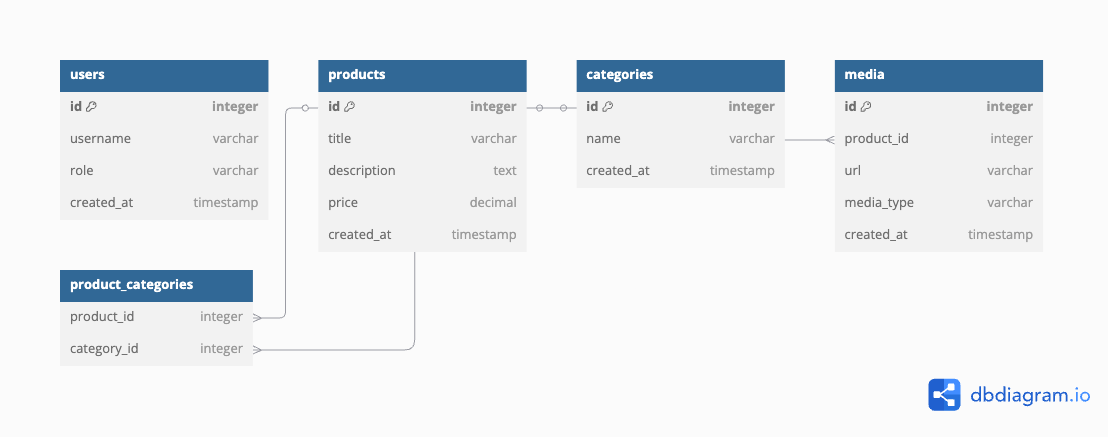
\includegraphics[width=0.7\textwidth]{img/erdSRSMRPL.png}
    \caption{ERD}
    \label{fig:erd}
\end{figure}

\section{Product Functions}
\begin{itemize}
    \item Product Presentation
    \begin{itemize}
        \item Display product categories
        \item Show product details (images, specifications, pricing)
        \\item Search and filtering functionality
    \end{itemize}
    
    \item WhatsApp Integration
    \begin{itemize}
        \item Pre-filled message templates for product inquiries
        \item Direct click-to-chat functionality
    \end{itemize}
    
    \item Admin Functions
    \begin{itemize}
        \item Add/remove products
        \item Update product information
        \item Manage product categories
        \item Manage communication with users
    \end{itemize}
\end{itemize}

\begin{figure}[H]
    \centering
    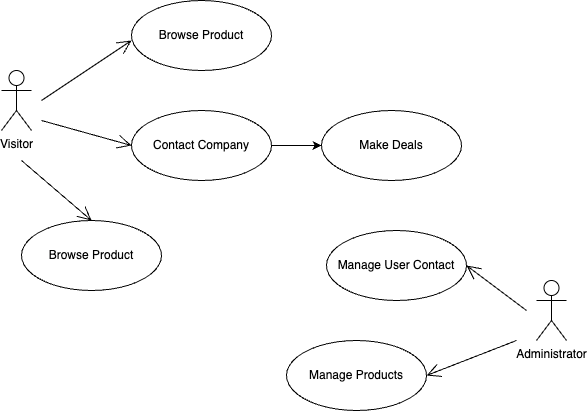
\includegraphics[width=0.5\textwidth]{img/usecaseSRS.png}
    \caption{Updated Use Case Diagram}
    \label{fig:usecase}
\end{figure}

\section{User Classes and Characteristics}
\begin{itemize}
    \item Website Visitors
    \begin{itemize}
        \item Frequency: Variable (casual browsing to serious buyers)
        \item Functions: Product browsing, WhatsApp contact
        \item Technical Expertise: Basic web navigation skills
    \end{itemize}
    
    \item Administrators
    \begin{itemize}
        \item Frequency: Daily updates
        \item Functions: Full product catalog management
        \item Security: Protected admin interface
    \end{itemize}
\end{itemize}

\section{Operating Environment}
\begin{itemize}
    \item Server Environment
    \begin{itemize}
        \item Web server with product database
        \item CMS for content management
    \end{itemize}
    
    \item Client Environment
    \begin{itemize}
        \item Modern web browsers
        \item Mobile-first responsive design
    \end{itemize}
    
    \item Database
    \begin{itemize}
        \item Relational database (MySQL/PostgreSQL)
        \item Cloud Bucket to store image blob (AWS S3 Bucket)
    \end{itemize}
\end{itemize}

\section{Design and Implementation Constraints}
\begin{itemize}
    \item Technical Constraints
    \begin{itemize}
        \item Responsive design requirements
        \item WhatsApp Business API integration
        \item Optimized media loading for product images
    \end{itemize}
    
    \item Performance Constraints
    \begin{itemize}
        \item Page load time <3s for 95\% of users
        \item Support 500 concurrent users
    \end{itemize}
    
    \item Security Constraints
    \begin{itemize}
        \item Secure admin interface
        \item Regular database backups
    \end{itemize}
\end{itemize}

\section{Assumptions and Dependencies}
\begin{itemize}
    \item Assumptions
    \begin{itemize}
        \item Users have WhatsApp installed
        \item Primary access via mobile devices
        \item Product availability matches physical inventory
    \end{itemize}
    
    \item Dependencies
    \begin{itemize}
        \item WhatsApp Business API availability
        \item Web hosting reliability
        \item Image CDN for product photos
    \end{itemize}
    
    \item Risks
    \begin{itemize}
        \item WhatsApp API changes
        \item Inventory discrepancies
        \item High bounce rates from casual browsers
    \end{itemize}
\end{itemize}

\chapter{External Interface Requirements}

\section{User Interfaces}
% $<$Describe the logical characteristics of each interface between the software 
% product and the users. This may include sample screen images, any GUI standards 
% or product family style guides that are to be followed, screen layout 
% constraints, standard buttons and functions (e.g., help) that will appear on 
% every screen, keyboard shortcuts, error message display standards, and so on.  
% Define the software components for which a user interface is needed. Details of the user interface design should be documented in a separate user interface 
% specification.$>$
\subsection{Landing Page}
\begin{figure}[H]
    \centering
    \begin{minipage}{0.4\textwidth}
        \centering
        \fbox{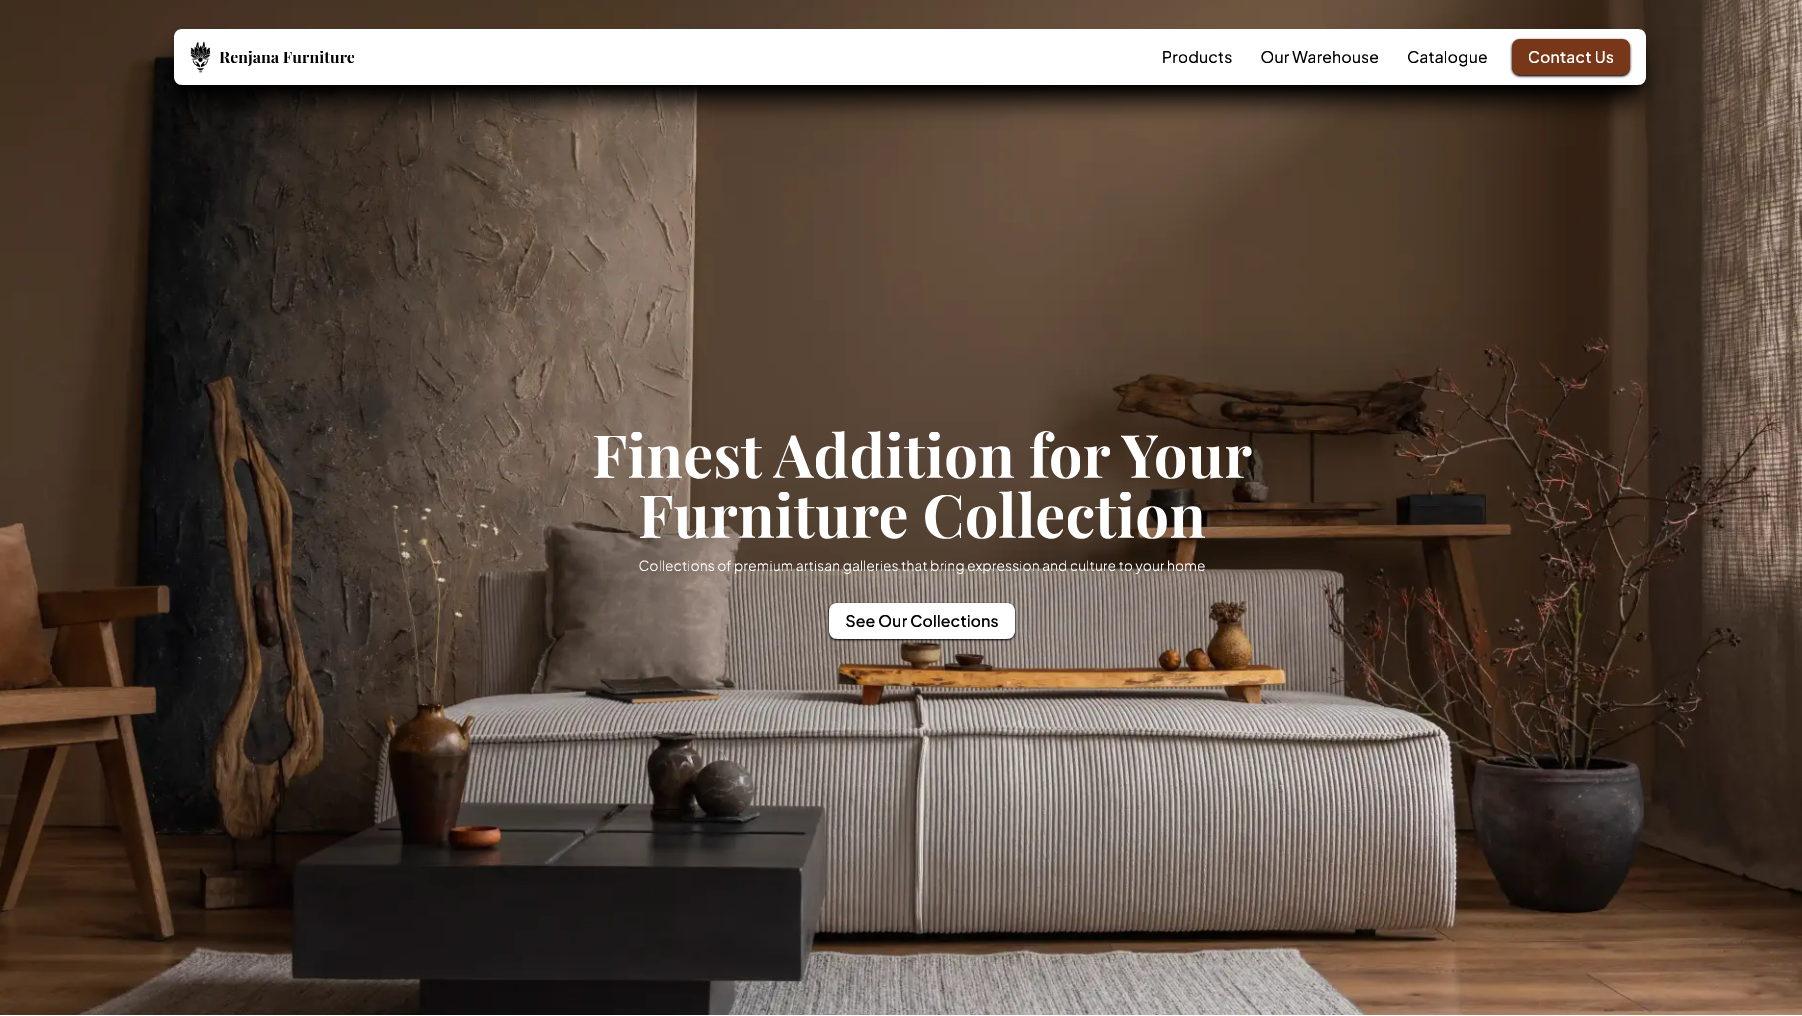
\includegraphics[width=\linewidth]{img/ui/landingpage-1.png}}
        \caption{Hero Section}
    \end{minipage}
    \hfill
    \begin{minipage}{0.5\textwidth}
        \centering
        \fbox{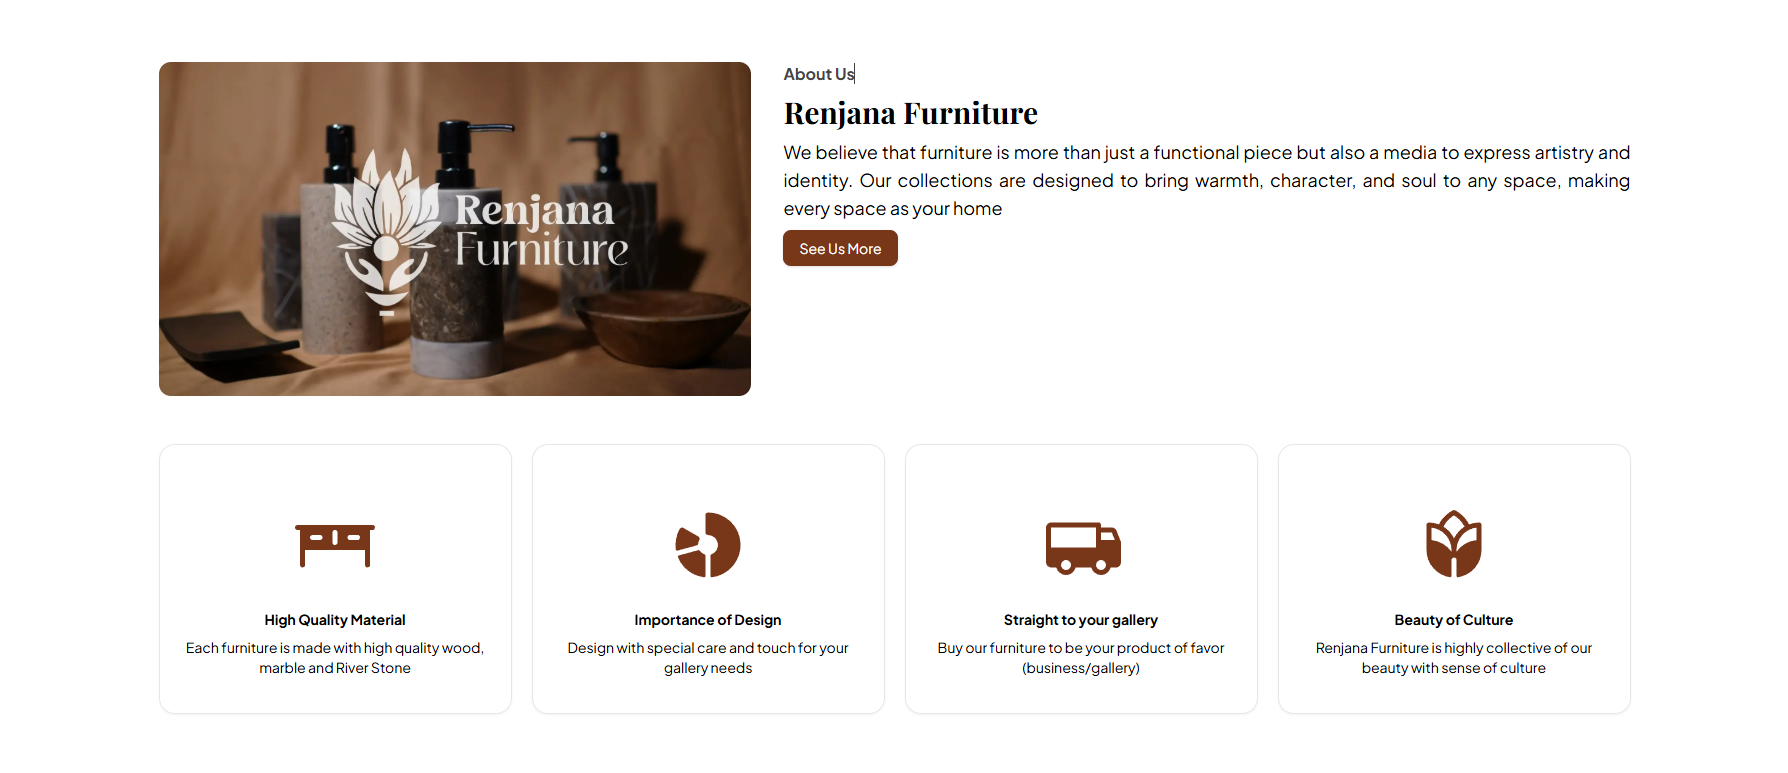
\includegraphics[width=\linewidth]{img/ui/landingpage-2.png}}
        \caption{About Section}
    \end{minipage}
\end{figure}
\begin{figure}[H]
    \centering
    \begin{minipage}{0.4\textwidth}
        \centering
        \fbox{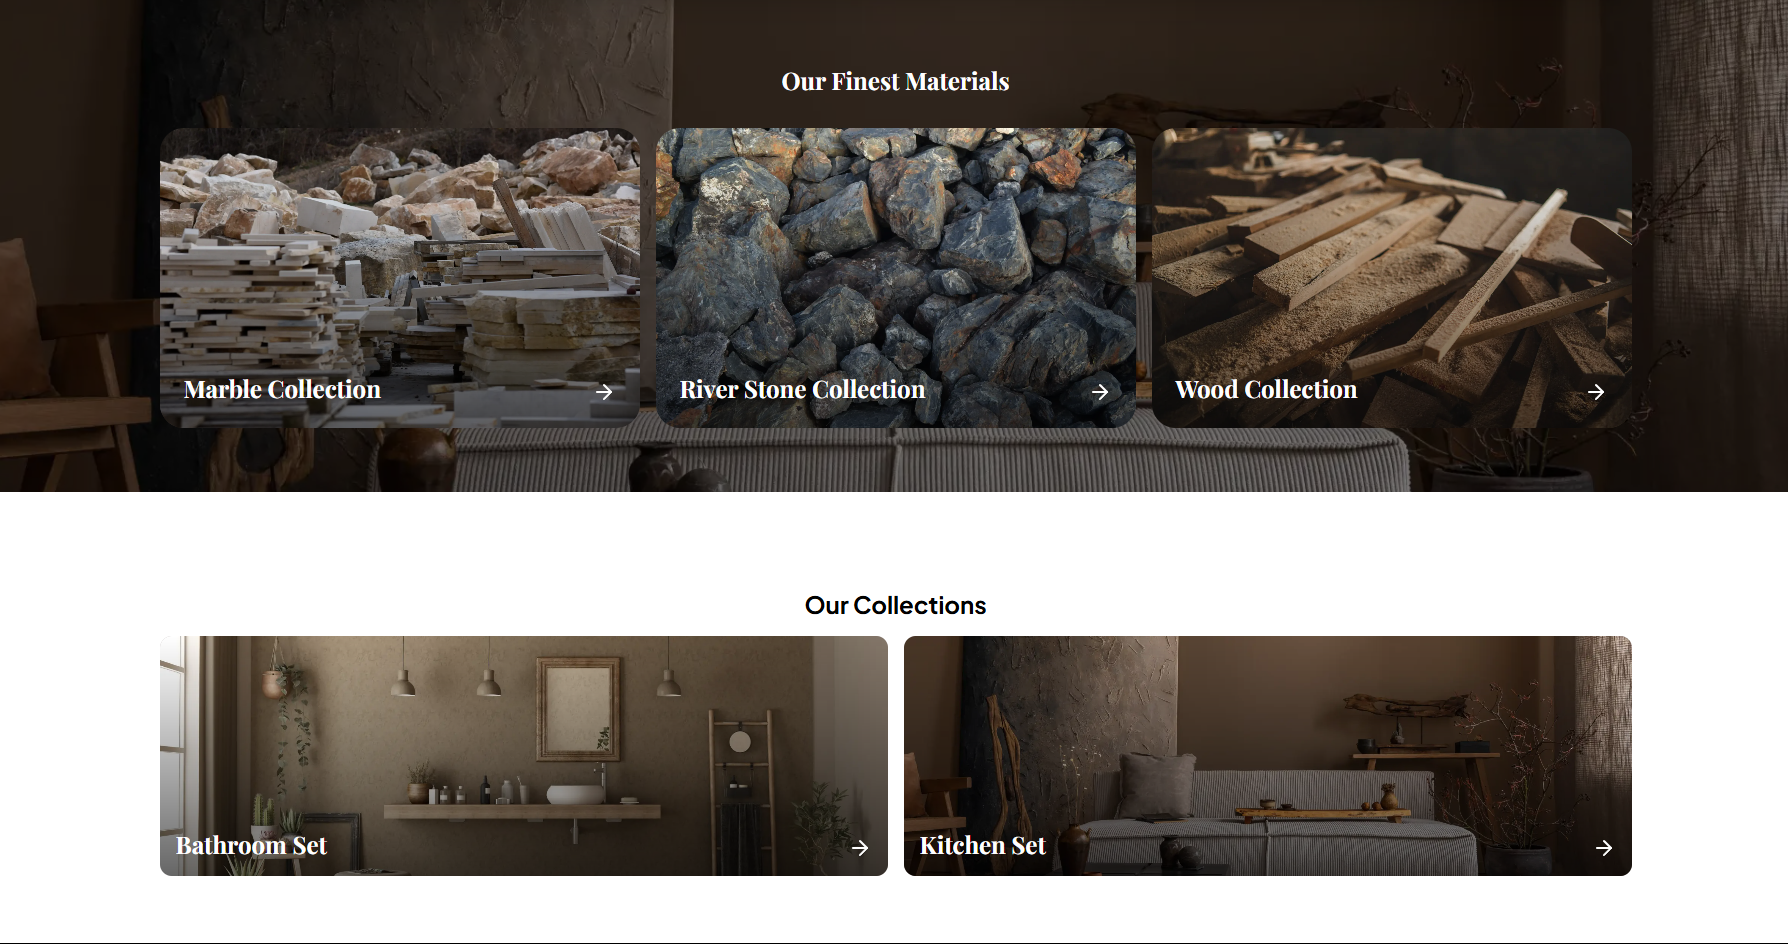
\includegraphics[width=\linewidth]{img/ui/landingpage-3.png}}
        \caption{collections Section}
    \end{minipage}
    \hfill
    \begin{minipage}{0.5\textwidth}
        \centering
        \fbox{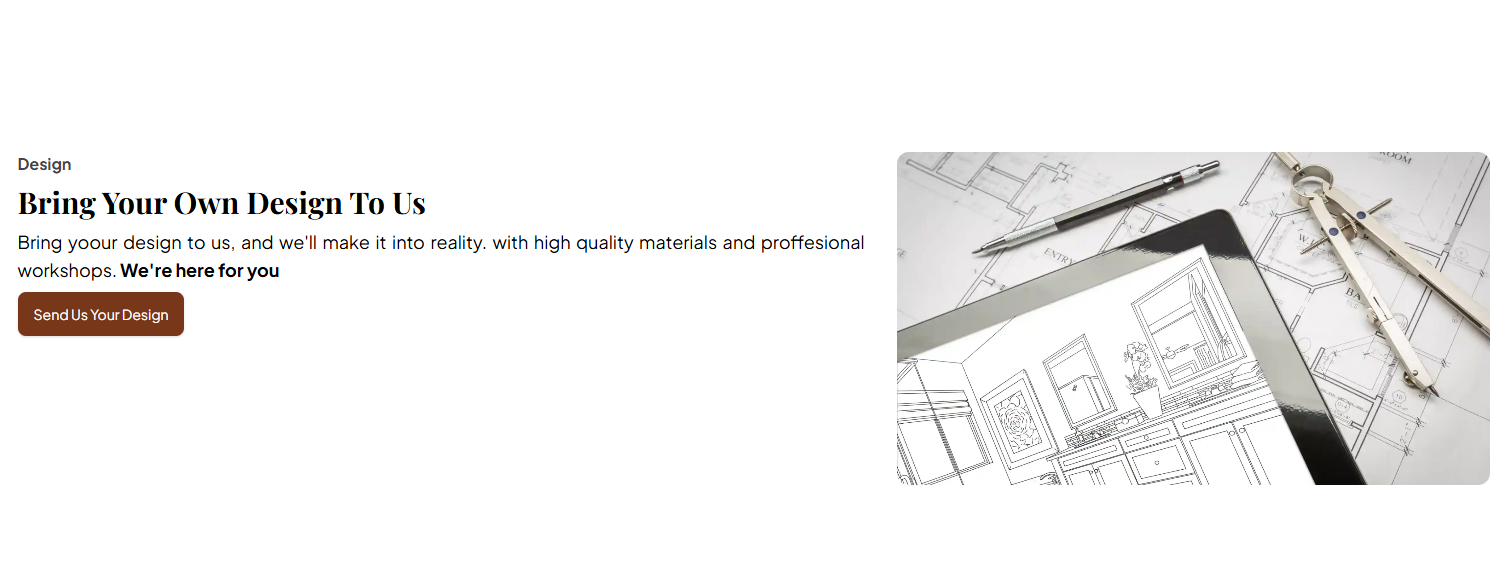
\includegraphics[width=\linewidth]{img/ui/landingpage-4.png}}
        \caption{Custom Design Section}
    \end{minipage}
\end{figure}

\begin{figure}[H]
    \centering
    \begin{minipage}{0.48\textwidth}
        \centering
        \fbox{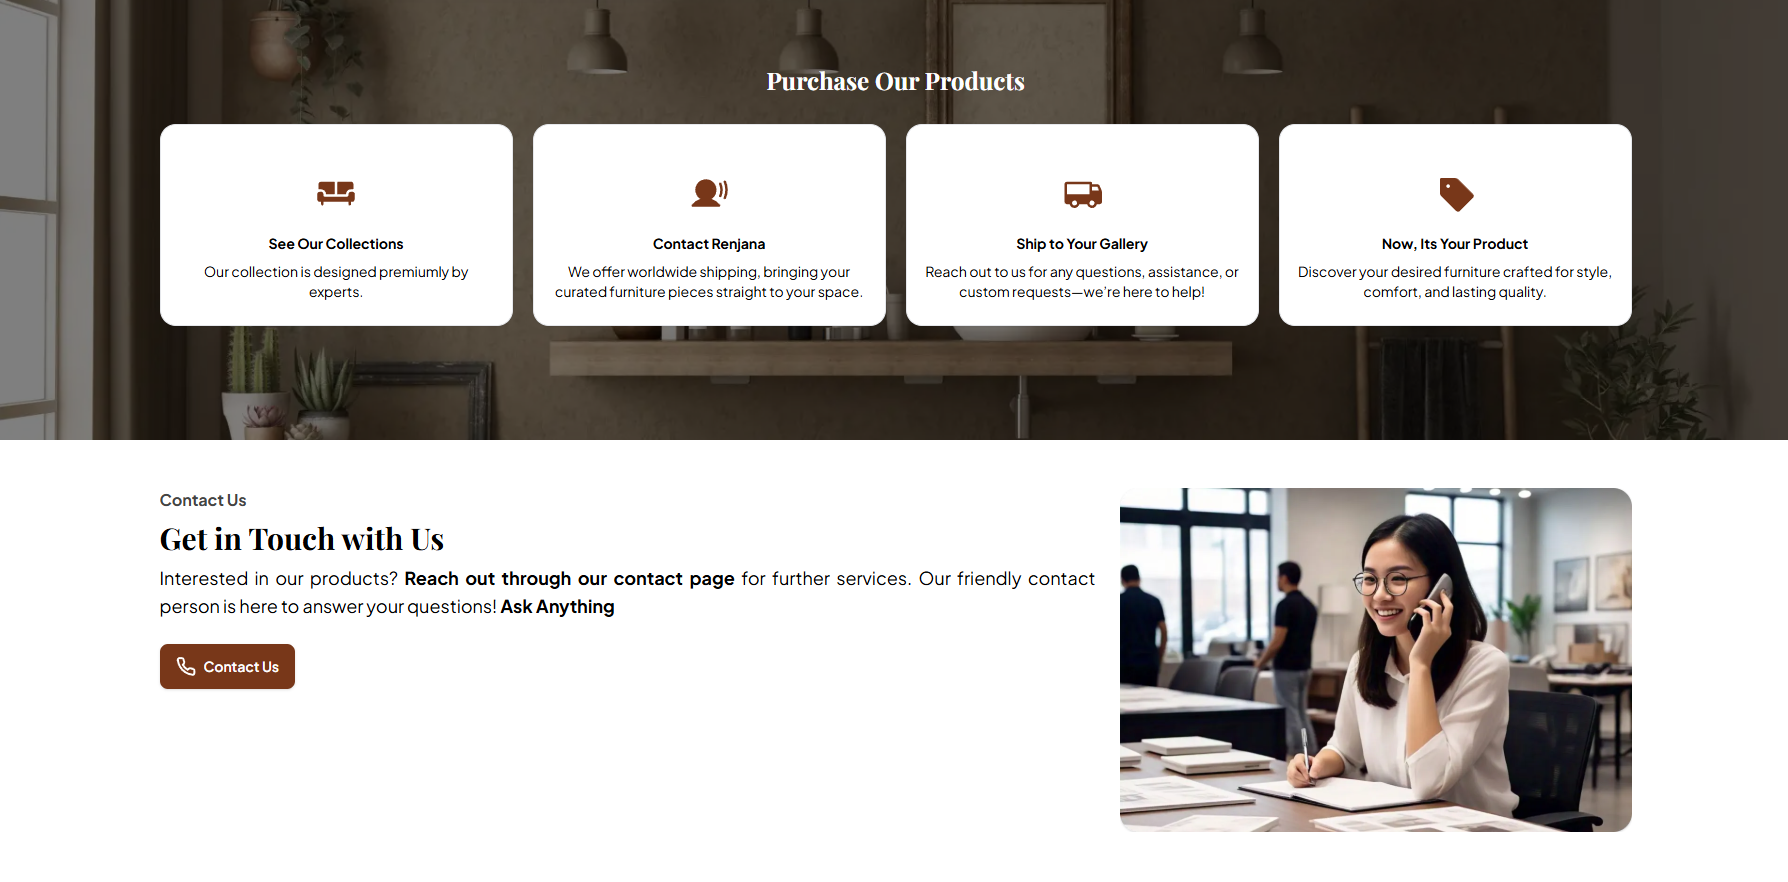
\includegraphics[width=\linewidth]{img/ui/landingpage-5.png}}
        \caption{Timeline and Contact Section}
    \end{minipage}
    \hfill
    \begin{minipage}{0.44\textwidth}
        \centering
        \fbox{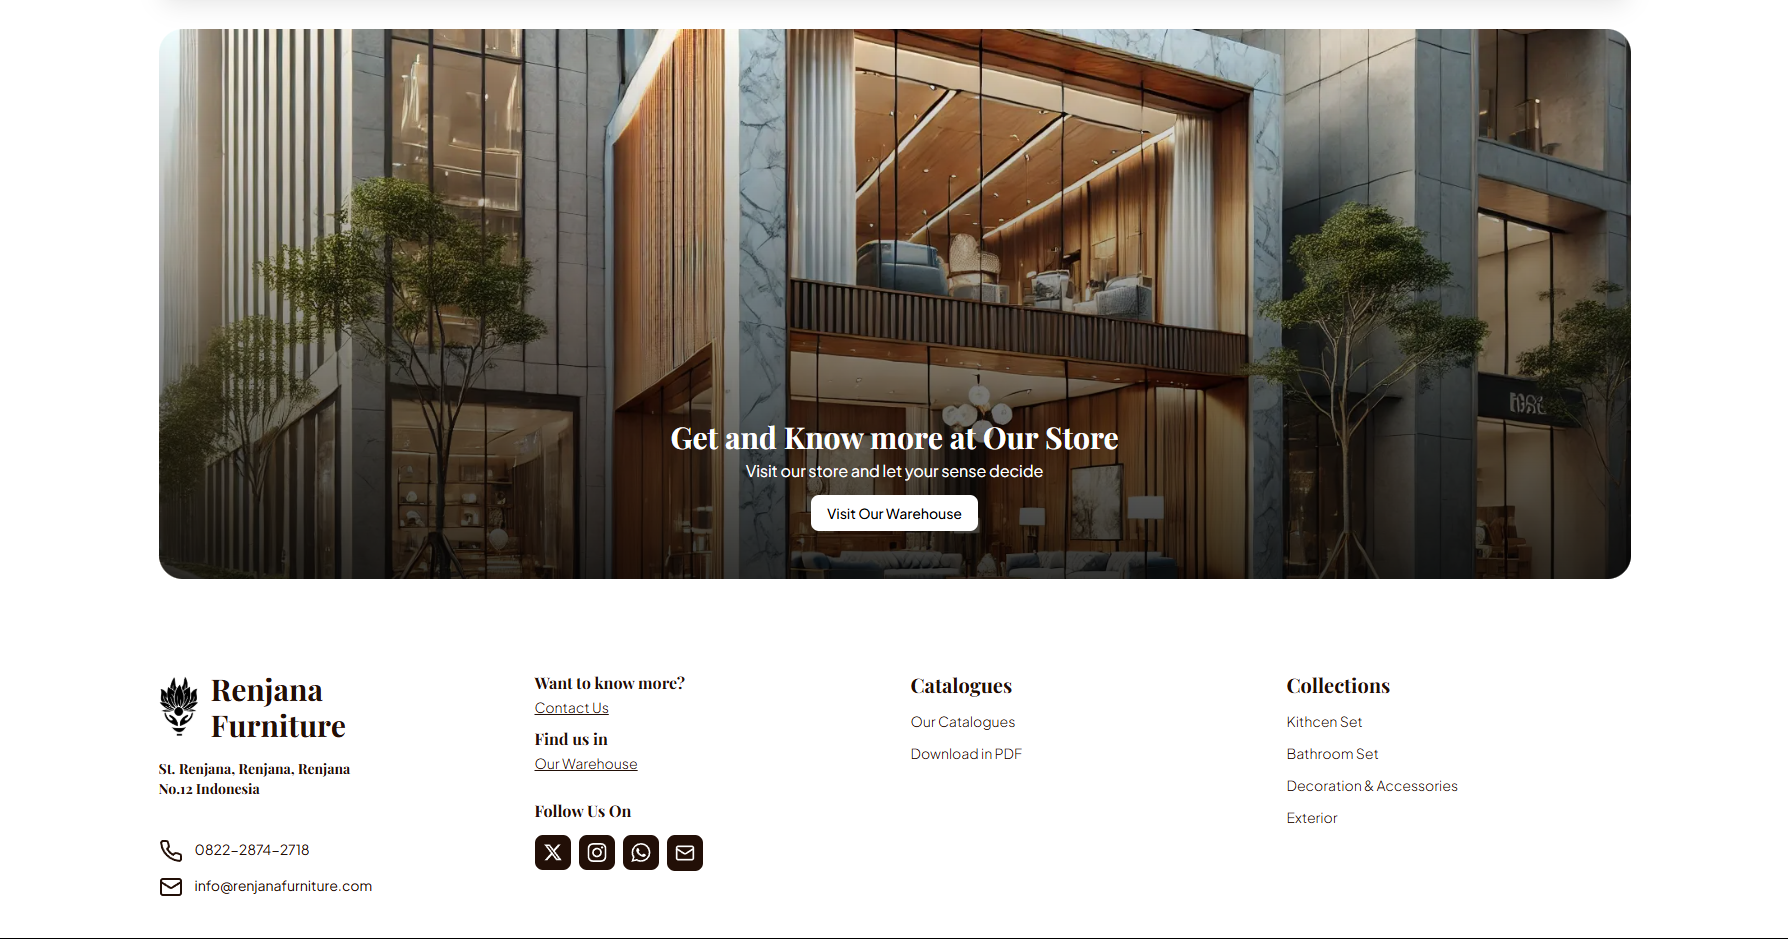
\includegraphics[width=\linewidth]{img/ui/landingpage-6.png}}
        \caption{CTA Section}
    \end{minipage}
\end{figure}

\begin{enumerate}
    \item[$\bullet$] First-time users accessing the website will land on this page.
    \item[$\bullet$] Displays an overview of the product catalog, key collections, and featured products.
    \item[$\bullet$] Includes navigation links to the catalog, collections, warehouse, and contact page.
    \item[$\bullet$] CTA buttons allow users to download the catalog, contact support, or browse collections.
\end{enumerate}

\subsection{Warehouse Page}
\begin{figure}[H]
    \centering
    \fbox{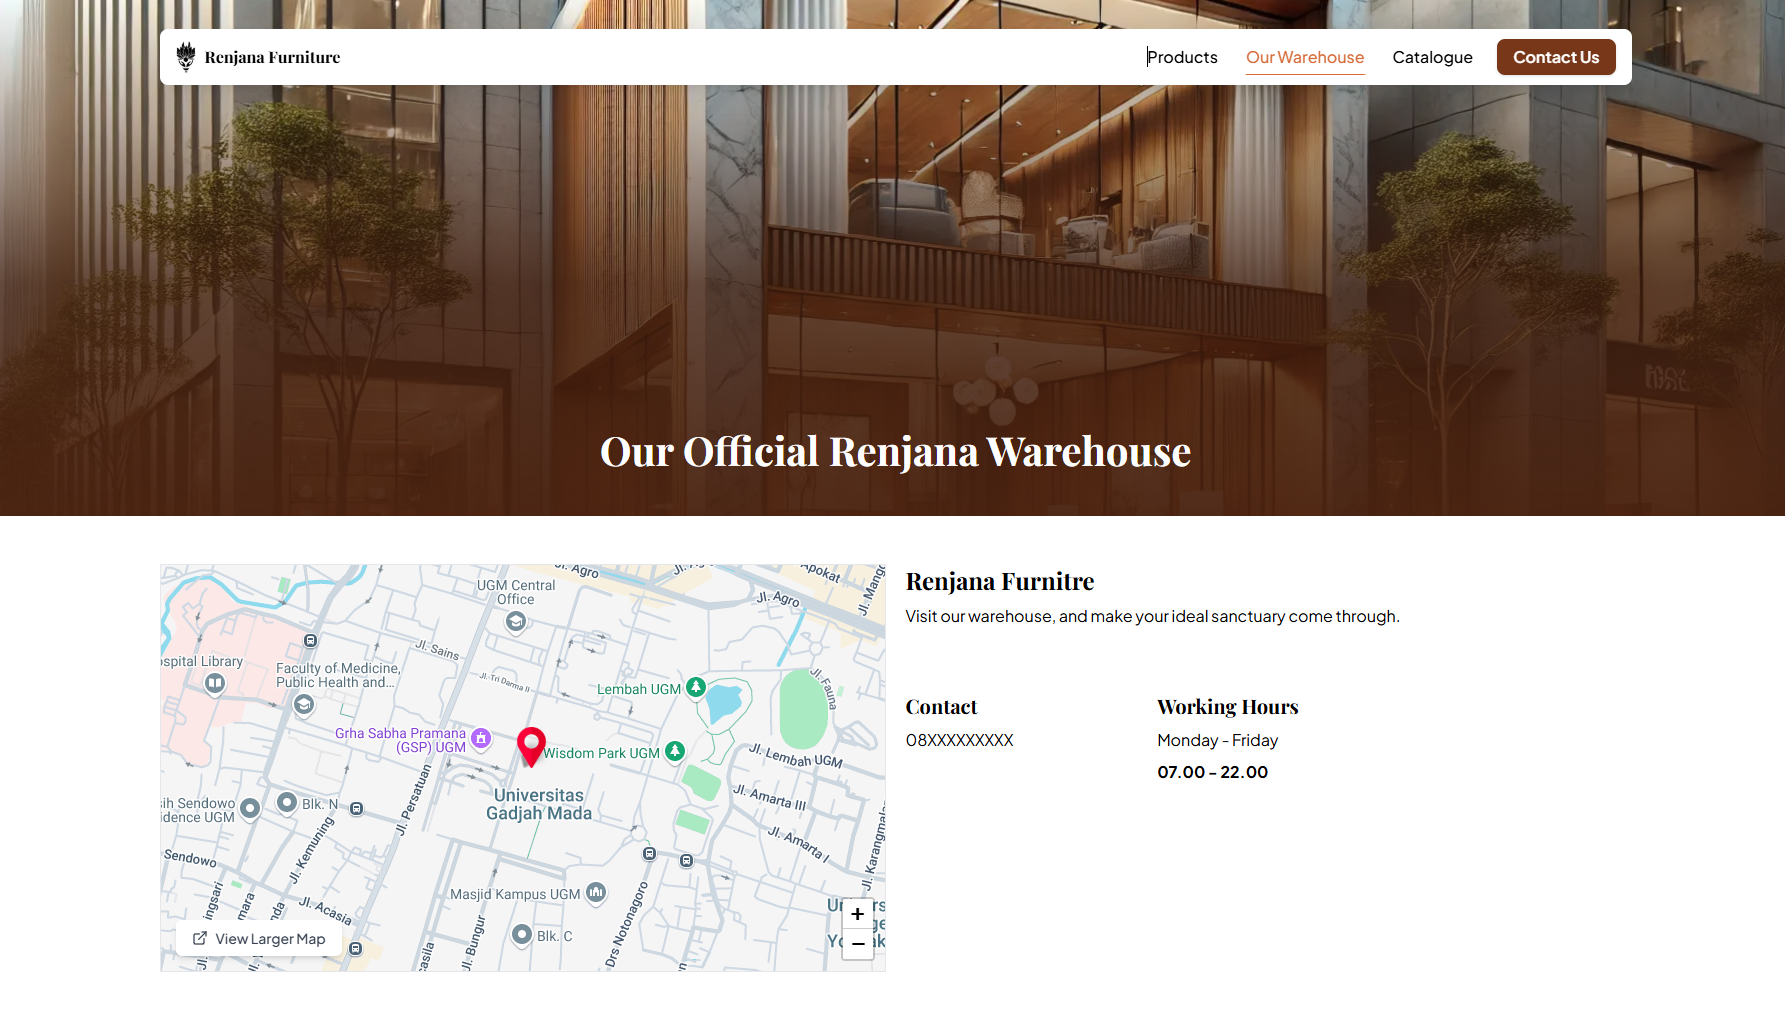
\includegraphics[width=0.7\linewidth]{img/ui/warehousepage.png}}
    \caption{Warehouse Page}
\end{figure}
\begin{enumerate}
    \item[$\bullet$] Shows the business’s warehouse/store location using Google Maps API.
    \item[$\bullet$] Displays the address and contact details.
    \item[$\bullet$] A CTA button allows users to open the location directly in Google Maps for navigation.
\end{enumerate}

\subsection{Catalogue Page}
\begin{figure}[H]
    \centering
    \fbox{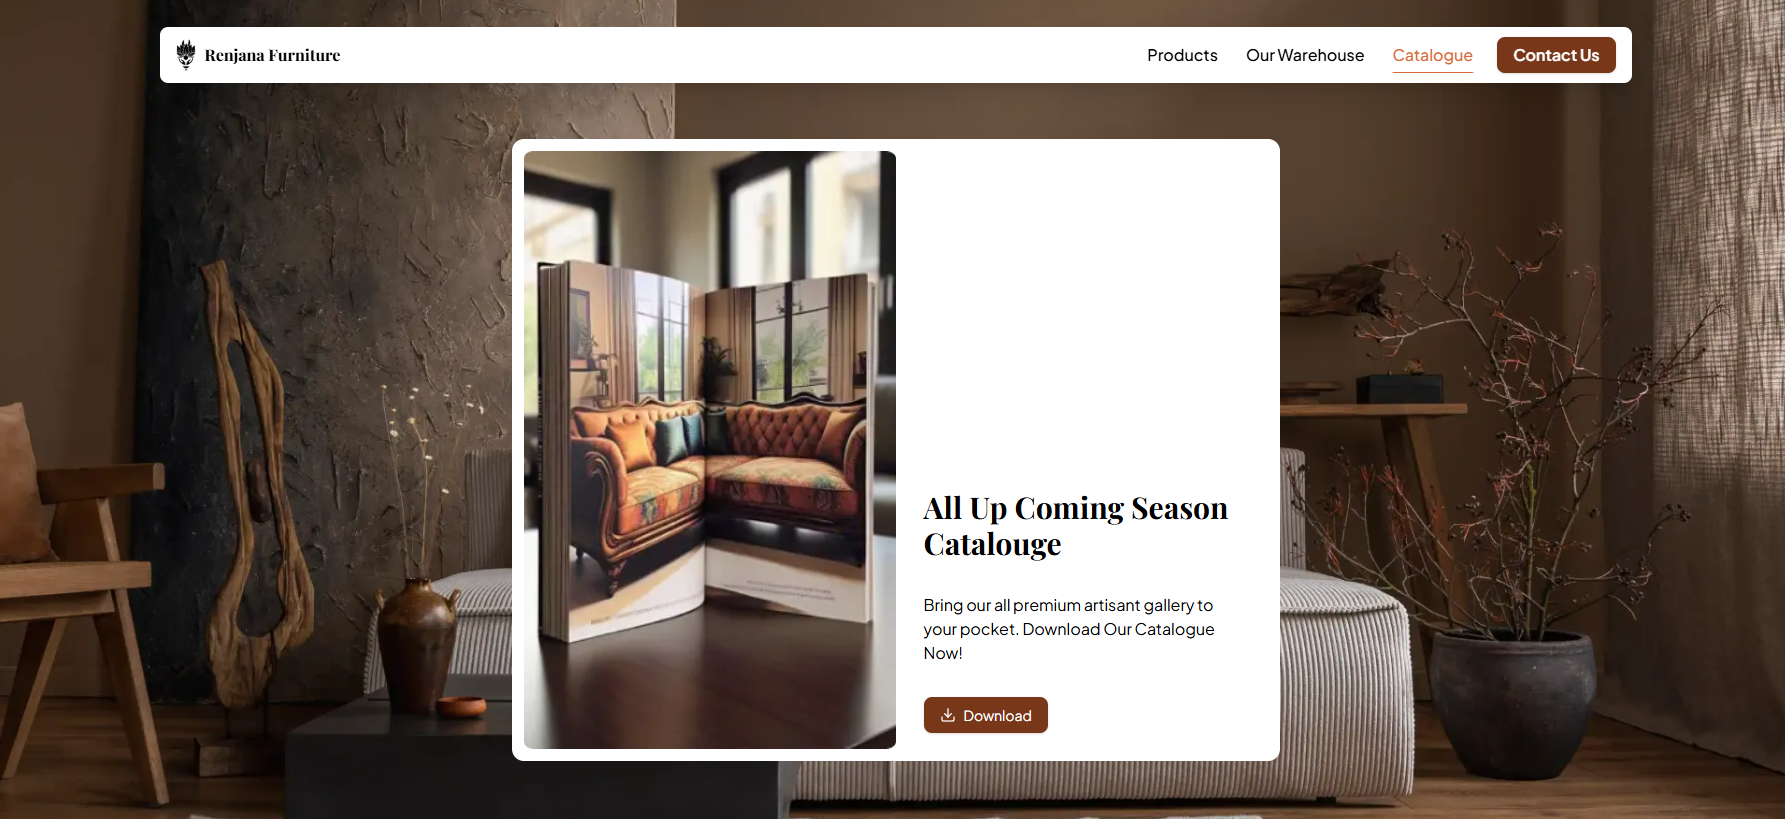
\includegraphics[width=0.7\linewidth]{img/ui/cataloguepage.png}}
    \caption{Catalogue Page}
\end{figure}
\begin{enumerate}
    \item[$\bullet$] Provides a dedicated section for users to download the latest catalog in PDF format.
    \item[$\bullet$] Includes a clear Download CTA button.
\end{enumerate}

\subsection{Collection Page}
\begin{figure}[H]
    \centering
    \fbox{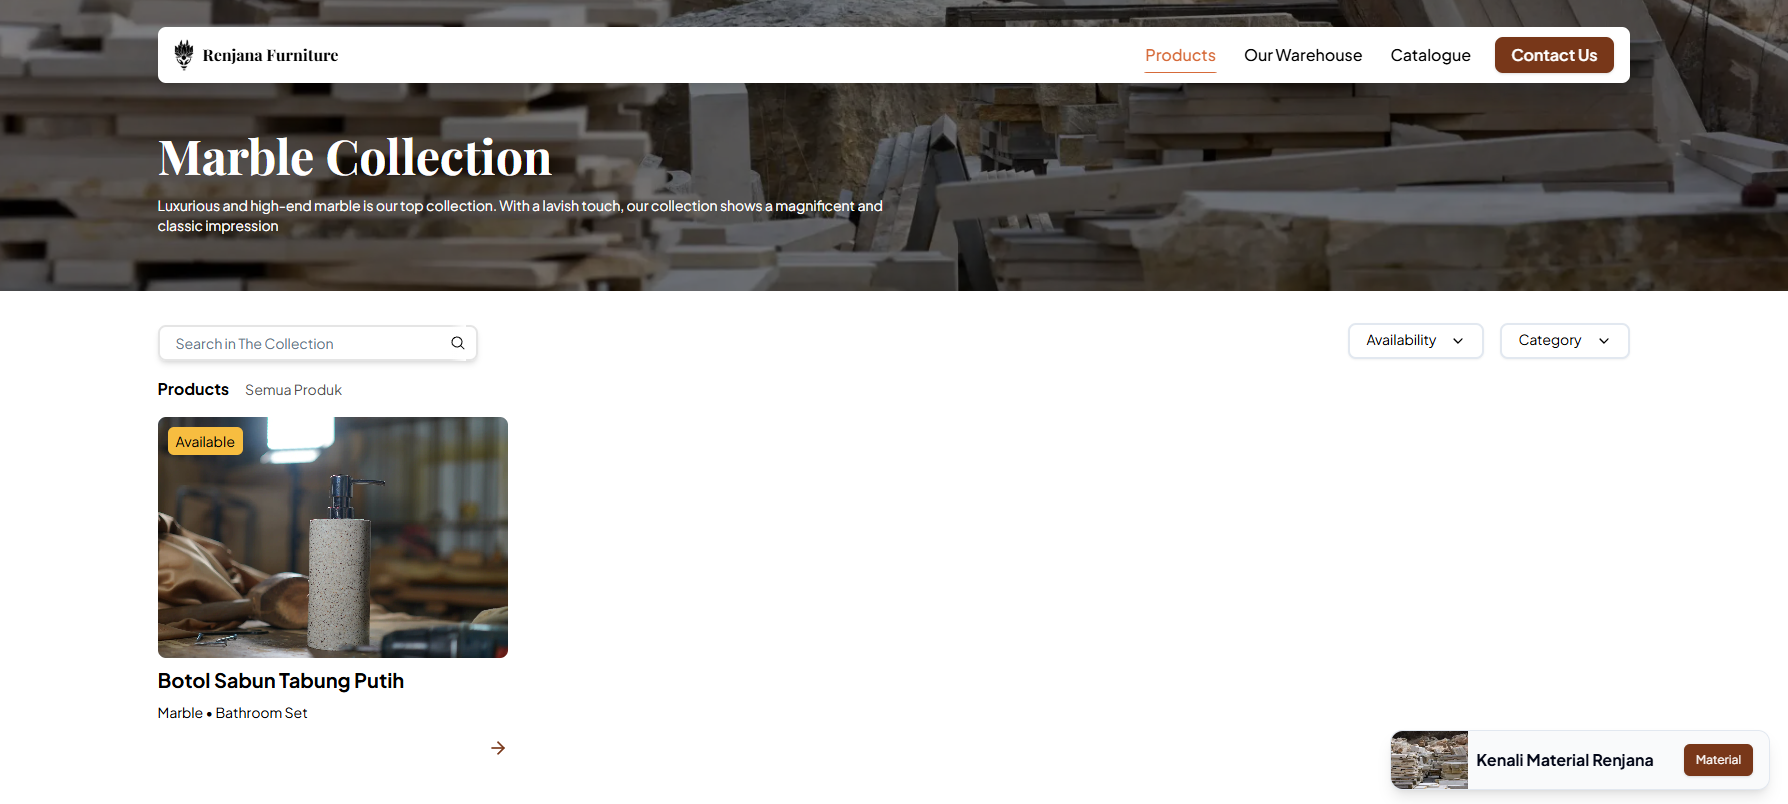
\includegraphics[width=0.7\linewidth]{img/ui/collectionpage.png}}
    \caption{Collection Page}
\end{figure}
\begin{enumerate}
    \item[$\bullet$] Displays product categories in two main sections:
    \begin{enumerate}
        \item Materials Collection (Wood, Marble, River Stone).
        \item Other Categories (Kitchen Set, Bathroom Set, Decoration & Accessories, Exterior).
    \end{enumerate}
    \item[$\bullet$] Users can filter and browse products based on selected categories.
\end{enumerate}

\subsection{Product Page}
\begin{figure}[H]
    \centering
    \fbox{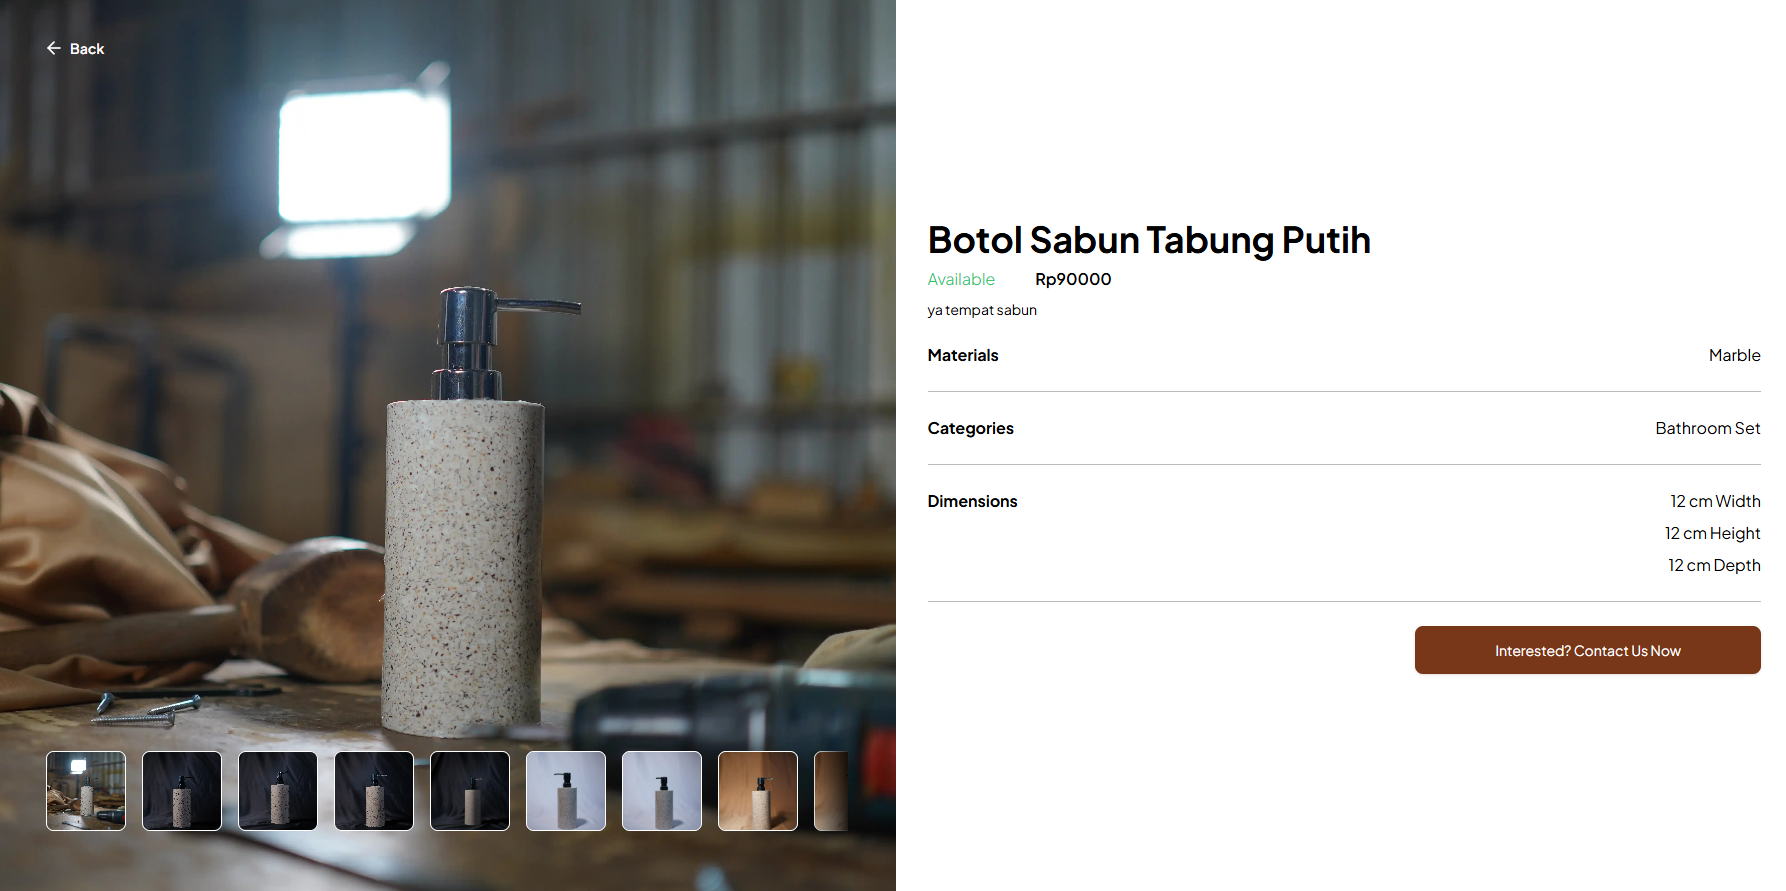
\includegraphics[width=0.7\linewidth]{img/ui/productpage.png}}
    \caption{Catalogue Page}
\end{figure}
\begin{enumerate}
    \item[$\bullet$] Displays product details, including:
    \begin{enumerate}
        \item Product images (stored in Supabase/Vercel Postgres).
        \item Name, description, dimensions (x, y, z), availability, and optional price.
    \end{enumerate}
    \item[$\bullet$] Users can contact the business via WhatsApp for further inquiries.
\end{enumerate}


% Done
\section{Hardware Interfaces}
The catalog website and the admin dashboard do not depend on specific hardware components, and therefore, no direct hardware interfaces are required. All product-related data, including images, descriptions, and other relevant details, are managed within the web platform. Payment transactions are facilitated through direct communication via WhatsApp rather than a dedicated payment processing hardware.

The database server connection is handled by the underlying infrastructure provided by the hosting service, ensuring reliable data storage and retrieval for both visitors and administrators. This approach abstracts hardware dependencies, allowing the system to operate efficiently across various environments.

% Done
\section{Software Interfaces}
The catalog website interacts with various software components to ensure seamless functionality and efficient data management. It is developed using Next.js as the primary frontend framework, with Tailwind CSS for styling and responsive design. The backend is managed through Payload CMS, which facilitates content organization and retrieval.

The system utilizes Supabase (Vercel Postgres) as its primary database for storing product details, user interactions, and other relevant data. Additionally, Supabase storage is used to handle and serve product images, ensuring optimized retrieval and delivery. Communication between the frontend and backend occurs via API requests, allowing structured data exchange and synchronization.

For transactions, the website does not include an integrated payment gateway but instead facilitates purchases through direct WhatsApp messaging. Furthermore, third-party libraries and services are integrated for image optimization, SEO enhancements, and performance monitoring to improve user experience and website visibility.

Data sharing between software components follows an API-driven approach, ensuring security, consistency, and scalability. If required, additional implementation constraints, such as authentication mechanisms and rate limiting, can be applied to protect data integrity.

% Done
\section{Communications Interfaces}
The catalog website relies on standard web communication protocols to ensure seamless data exchange between the frontend, backend, and external services. The system primarily uses HTTPS for secure communication and is accessible through modern web browsers.

Data transactions between the frontend and backend are managed through GraphQL API provided by Payload CMS, allowing efficient retrieval and management of product information stored in Supabase (Vercel Postgres).

For customer inquiries via the Contact Us form, the system integrates with Google Sheets API to store submitted form data in a centralized Google Sheet. Additionally, Nodemailer is used to send email notifications based on form submissions, ensuring that administrators are promptly informed of customer inquiries.

To enhance the user experience, the website also integrates Google Maps API, which provides an interactive map displaying the warehouse location. This allows users to easily locate the company's physical store or storage facility.

Since transactions are conducted outside the platform via WhatsApp messaging, no payment gateway integration is required. WhatsApp's built-in encryption ensures secure communication between customers and the business.

To maintain data integrity and security, all API communications follow industry best practices, including authentication mechanisms, rate limiting, and encrypted data transmission where applicable.

\chapter{System Features}
% Upper Bound
% $<$This template illustrates organizing the functional requirements for the 
% product by system features, the major services provided by the product. You may 
% prefer to organize this section by use case, mode of operation, user class, 
% object class, functional hierarchy, or combinations of these, whatever makes the 
% most logical sense for your product.$>$

% \section{System Feature 1}
% $<$Don’t really say “System Feature 1.” State the feature name in just a few 
% words.$>$

% \subsection{Description and Priority}
% $<$Provide a short description of the feature and indicate whether it is of 
% High, Medium, or Low priority. You could also include specific priority 
% component ratings, such as benefit, penalty, cost, and risk (each rated on a 
% relative scale from a low of 1 to a high of 9).$>$

% \subsection{Stimulus/Response Sequences}
% $<$List the sequences of user actions and system responses that stimulate the 
% behavior defined for this feature. These will correspond to the dialog elements 
% associated with use cases.$>$

% \subsection{Functional Requirements}
% $<$Itemize the detailed functional requirements associated with this feature.  
% These are the software capabilities that must be present in order for the user 
% to carry out the services provided by the feature, or to execute the use case.  
% Include how the product should respond to anticipated error conditions or 
% invalid inputs. Requirements should be concise, complete, unambiguous, 
% verifiable, and necessary. Use “TBD” as a placeholder to indicate when necessary 
% information is not yet available.$>$

% $<$Each requirement should be uniquely identified with a sequence number or a 
% meaningful tag of some kind.$>$

% REQ-1:	REQ-2:

% Lower Bound

\section{Product Management}

\subsection{Description and Priority}
This feature enables administrators to efficiently manage the product catalog by adding, editing, and deleting products. Each product entry includes essential details such as name, description, availability status, dimensions (X, Y, Z), category, and optional pricing. Additionally, product images are stored securely in Supabase (Vercel Postgres). Given its critical role in maintaining the catalog, this feature is assigned high priority.

\subsection{Stimulus/Response Sequences}
\begin{enumerate}
    \item The admin logs into the dashboard or admin panel.
    \item The admin selects Add Product, fills in the product form, and submits it.
    \item The system stores the data in the database via Payload CMS.
    \item The admin selects Edit Product, modifies the details, and saves the changes.
    \item The system updates the product data in the database.
    \item The admin selects Delete Product, and the system removes the product from the database.
\end{enumerate}

\subsection{Functional Requirements}
\begin{enumerate}
    \item[$\bullet$] REQ-1: The system must provide an admin dashboard to manage products.
    \item[$\bullet$] REQ-2: The system must support CRUD (Create, Read, Update, Delete) operations for products.
    \item[$\bullet$] REQ-3: Product images must be stored and retrieved from Supabase (Vercel Postgres).
    \item[$\bullet$] REQ-4: The system must display error messages for invalid inputs.
\end{enumerate}

\section{Product Catalogue Display}

\subsection{Description and Priority}
This feature ensures that products in the catalog are displayed in an organized manner based on predefined collections. The catalog is structured into two main categories:
\begin{enumerate}
    \item Materials Collection: Includes products categorized by material, such as Wood, Marble, and River Stone.
    \item Other Categories: Groups products based on their function or placement, including **Kitchen Set, Bathroom Set, Decoration & Accessories, and Exterior.
\end{enumerate}
This feature is high priority, as it directly impacts the browsing experience and usability of the catalog for customers.

\subsection{Stimulus/Response Sequences}
\begin{enumerate}
    \item User Action: Opens the catalog landing page.
    \begin{enumerate}
        \item[$\bullet$] System Response: Displays collections section and navigation bar with   various predefined collections with a categorized product listing.
    \end{enumerate}
    \item User Action: Selects a collection (e.g., "Wood" or "Kitchen Set").
    \begin{enumerate}
        \item[$\bullet$] System Response: Filters and presents products from the selected collection.
    \end{enumerate}
    \item User Action: Clicks on a product to view its details.
    \begin{enumerate}
        \item[$\bullet$] System Response: Displays the product’s name, description, dimensions, availability status, images, and optional price.
    \end{enumerate}
\end{enumerate}

\subsection{Functional Requirements}
\begin{enumerate}
    \item[$\bullet$] REQ-5: The system must categorize products into Materials Collection and Other Categories.
    \item[$\bullet$] REQ-6: The catalog page must display collections in a structured manner.
    \item[$\bullet$] REQ-7: Users must be able to filter products by collection.
    \item[$\bullet$] REQ-8: The system must provide a detailed product view when a user selects a product.
\end{enumerate}

\section{Contact Form Submission}

\subsection{Description and Priority}
This feature allows users to submit inquiries or information requests via the contact form. Data is stored in Google Sheets API, and the admin receives email notifications via Nodemailer. This feature has a medium priority.

\subsection{Stimulus/Response Sequences}
\begin{enumerate}
    \item User Action: Fills out the contact form and clicks Submit.
    \begin{enumerate}
        \item[$\bullet$] System Response: Stores the data in Google Sheets API.
    \end{enumerate}
    \item System Action: Sends an email notification to the admin using Nodemailer.
    \item User Action: Receives a confirmation message indicating that the inquiry was successfully submitted.
\end{enumerate}

\subsection{Functional Requirements}
\begin{enumerate}
    \item[$\bullet$] REQ-8: The contact form must store submissions in Google Sheets API.
    \item[$\bullet$] REQ-10: The system must send email notifications to the admin via Nodemailer.
    \item[$\bullet$] REQ-11: The system must display a confirmation message after form submission.
\end{enumerate}

\section{Warehouse Location Display}

\subsection{Description and Priority}
This feature displays the warehouse/store location using Google Maps API, allowing users to easily find the business’s physical address. This feature has a low priority, but it enhances the user experience.

\subsection{Stimulus/Response Sequences}
\begin{enumerate}
    \item User Action: Opens the warehouse location page.
    \begin{enumerate}
        \item[$\bullet$] System Response: Displays the warehouse address along with a map preview.
    \end{enumerate}
    \item User Action: Clicks the CTA button to open the location.
    \begin{enumerate}
        \item[$\bullet$] System Response: Redirects the user to Google Maps, opening the coordinates in the app or web version.
    \end{enumerate}
\end{enumerate}

\subsection{Functional Requirements}
\begin{enumerate}
    \item[$\bullet$] REQ-12: The system must display the warehouse location on a map.
    \item[$\bullet$] REQ-13: The system must provide a CTA button that allows users to open the location in Google Maps.
    \item[$\bullet$] REQ-14: Clicking the CTA button must redirect users to Google Maps with the correct coordinates.
\end{enumerate}

% dsa


\chapter{Other Nonfunctional Requirements}

\section{Performance Requirements}

The AAA Furnitures web app must ensure efficient performance under various conditions to enhance the user experience and support business operations.

\begin{itemize}
\item \textbf{Page Load Speed}: All web pages should achieve a Largest Contentful Paint (LCP) of under 2.5 seconds and a First Contentful Paint (FCP) of under 1.8 seconds under standard network conditions.
\item \textbf{Search and Filtering}: The product search and filtering functions should return results within 2 seconds to ensure seamless navigation.
\item \textbf{Image Optimization}: Product images must be served in WebP format and lazy-loaded to ensure they load in under 2 seconds.
\item \textbf{API Performance}: Backend APIs should respond within 200ms to ensure smooth interaction between frontend and backend components.
\item \textbf{Database Queries}: Queries should be optimized to execute within 100ms to prevent bottlenecks.
\end{itemize}

\section{Safety Requirements}
Safety measures are essential to protect user data and ensure proper handling of catalogue data.

\begin{itemize}
\item \textbf{Error Handling}: The system should provide informative error messages and prevent crashes or unresponsive states when encountering unexpected user input. A dedicated 404 Error page is required.
\item \textbf{Backup and Recovery}: Regular backups must be maintained to prevent data loss due to system failures.
\item \textbf{Product Descriptions and Pricing}: The administrators must verify that product descriptions and pricing updates do not result in discrepancies that may mislead customers.
\end{itemize}

\section{Security Requirements}
Security measures focus on protecting user data and preventing unauthorized access.

\begin{itemize}
\item \textbf{Admin Panel Security}: The admin panel is only accessible via a designated URL path (/admin) and requires authentication to prevent unauthorized modifications.
\item \textbf{HTTPS Compliance}: The web app enforces HTTPS to encrypt all communications between users and the server, ensuring secure transactions.
\item \textbf{Database Security}: Supabase policies are implemented to restrict unauthorized access and ensure only authenticated users can perform certain operations.
\item \textbf{Rate Limiting}: API rate limits should be enforced to mitigate abuse and prevent denial-of-service attacks.
\end{itemize}

\section{Software Quality Attributes}
The AAA Furnitures web app should adhere to high-quality software standards to enhance usability, maintainability, and reliability.

\begin{itemize}
\item \textbf{Usability}: The interface should be intuitive, ensuring users can browse, search, and complete purchases with minimal effort.
\item \textbf{Reliability}: The system should achieve at least 99.5\% uptime to ensure availability for customers.
\item \textbf{Scalability}: The application must be scalable to accommodate increased traffic and inventory expansion without performance degradation.
\item \textbf{Maintainability}: The codebase should be modular and well-documented to allow for future enhancements and bug fixes.
\item \textbf{Compatibility}: The web app should be compatible with major web browsers (Chrome, Firefox, Safari, Edge) and mobile devices.
\end{itemize}

\section{Business Rules}
The AAA Furnitures web app must follow operational principles that dictate how different roles interact with the system.

\begin{itemize}
\item \textbf{User Roles}: The system supports different roles such as customers and administrators. Customers do not need to create an account and can browse products and place orders, while administrators can manage inventory, orders via the admin panel.
\item \textbf{Inventory Management}: Only authorized administrators can add, update, or remove products from the inventory.
\item \textbf{Customer Support}: Users should be able to submit inquiries or complaints through a dedicated support line, either through WhatsApp or email linked on the footer of the website.
\end{itemize}

\phantomsection
\cleardoublepage
\addcontentsline{toc}{chapter}{\indexname}
\printindex
\end{document}
